\documentclass[a4paper,14pt]{extarticle}
\usepackage[left=2.5cm, right=1.5cm, vmargin=2.5cm]{geometry}
\usepackage[utf8]{inputenc}
\usepackage[T2A]{fontenc}
\usepackage[russian]{babel}
\usepackage{graphicx}
\graphicspath{{pictures/}}
\usepackage{caption}
\usepackage{subcaption}
\usepackage{indentfirst}
\setlength\parindent{5ex}
\usepackage{fancyhdr}
\usepackage{booktabs}
\usepackage{siunitx} 
\usepackage{pgfplotstable}
\usepackage{amsmath}
\usepackage{autonum}
\usepackage{amsfonts}
\DeclareMathOperator{\sign}{sgn}
\newcommand{\gt}{\textgreater} % знак больше
\newcommand{\lt}{\textless}       % знак меньше
\DeclareGraphicsExtensions{.pdf,.png,.jpg}
\pagestyle{fancy}
\fancyhf{}
\rhead{\thepage}
\renewcommand{\headrulewidth}{0pt}

\fancypagestyle{plain}{ 
	\fancyhf{}
	\rhead{\thepage}}

\author{Никитин Илья}

\title{Отчет по лабораторной работе №1: "Изучение поляризованного света"}
\date{\today}

\begin{document}
	
	\maketitle
	\tableofcontents

	\section{Задачи}
		Познакомиться с практическими аспектами работы с оптическим оборудованием, изучить различные виды поляризации, доказать формулы Френеля и закон Малюса
	\section{Оборудование}
		\begin{itemize}
			\item Лазер с длиной волны испускаемого света 532 нм
			\item Два линейных поляризатора
			\item Пластинки $\lambda$/2 и $\lambda$/4
			\item Стеклянная пластинка
			\item Черное зеркало
			\item Анализатор интенсивности падающего света
			\item Вращающаяся платформа с лапкой для закрепления пластинки или зеркала
			\item Различная оптическая арматура
		\end{itemize}
	\section{Теория}
		\subsection{Виды поляризации}
			Свет — это электромагнитная волна. Такие волны - поперечные, в них направления векторов $E$ и $H$ взаимно перпендикулярны и располагаются в плоскости, перпендикулярной направлению распространения волны. При этом положение векторов $E$ и $H$ в световой волне в пространстве может различным образом меняться со временем. Характер этого изменения говорит о поляризации света. Далее, для простоты будем следить только за вектором электрического поля $E$. 
			
			В простейшем случае направление вектора $E$ в пространстве может меняться со временем случайным образом. Это справедливо для большинства обычных источников света, в которых излучение создается большим количеством некогерентно испускающих свет атомов. В таком случае говорят об естественном или неполяризованном свете. 
			
			Возможен также случай, когда ориентация вектора $E$ не меняется со временем. Такой свет называется линейно поляризованным или, иначе, плоско поляризованным. В линейно поляризованной волне плоскость, в которой находятся вектор E и вектор направления распространения волны, называется плоскостью колебаний. 
			
			Колебания электрического поля в плоско поляризованной волне можно разложить на две взаимно перпендикулярных компоненты. В этом случае сдвиг фаз между колебаниями каждой из компонент равен нулю (или целому кратному $\pi$). Однако, в самом общем случае, сдвиг фаз между ними может быть произвольным, тогда вектор $E$ со временем будет описывать эллипс в пространстве. В этом случае говорят об эллиптически поляризованном свете. Если разность фаз колебаний составляет $\pi/2$ (или кратен $\pi/2$), вектор $E$ описывает окружность и в этом случае говорят о круговой поляризации света. 
			
			С течением времени направление вектора электрического поля в эллиптически поляризованной волне может вращаться как правосторонний винт, так и как левосторонний. Соответственно, в первом случае говорят о правой поляризации, а во втором о левой поляризации. При этом говорят о направлении поляризации. Заметим, однако, что к подобным терминам следует относится с осторожностью, так как в различных источниках направления поляризации могут быть определены по разному. 
			
			Важно отметить отличие между эллиптически поляризованного и неполяризованного света. Несмотря на то, что в обоих случаях наблюдаются колебания электрического поля в	любых взаимно перпендикулярных направлениях, в первом случае эти колебания происходят согласованно, с фиксированной разностью фаз. Во втором же случае эти колебания не согласованы. 
			
			Если свет является суммой неполяризованного и линейно поляризованного, то его можно охарактеризовать степенью поляризации $P$, которой называется величина:
			
			\begin{equation}
				P = \frac{I_{max} - I_{min}}{I_{max} + I_{min}},
			\end{equation}
			
			где $I_{max}$ и $I_{min}$ – максимальная и минимальная интенсивности частично поляризованного света, пропускаемого анализатором. Для естественного света она равна 0, для плоско	поляризованного 1. Эллиптически поляризованный свет этой величиной характеризовать не принято.
			
			\subsection{Поляризаторы и закон Малюса}
			Плоско поляризованный свет обычно получают с помощью специальных устройств — поляризаторов. После прохождения естественного света через поляризатор, получается линейно поляризованный свет. Направление колебаний электрического вектора в полученном линейно поляризованном свете называется разрешенным направлением поляризатора. Также поляризатор можно использовать не только для получения свет	определенной поляризации, но и для определения его поляризации. В этом случае поляризатор могут называть анализатором. 
			
			Интенсивность линейно поляризованного света $I_0$, после прохождения через анализатор, разрешенное направление которого составляет угол $\alpha$ к плоскости колебаний, задается законом Малюса:
			
			\begin{equation}
				I = I_0 \cos^2{\alpha}.
			\end{equation}
			
			Существует несколько способов получения плоско поляризованного света. На практике часто используются поляризаторы, чей принцип действия основан на явлении дихроизма, состоящее в различном поглощении света веществом в зависимости от поляризации. У некоторых кристаллов (например, у турмалина) различие коэффициента поглощения для света с перпендикулярными направлениями поляризации может быть настолько сильным, что даже при небольшой толщине кристалла при прохождении поглощается полностью одна из компонент. В итоге, на выходе получается линейно поляризованный свет.
			
			Кроме коэффициента поглощения для разных поляризаций может быть различным коэффициент преломления среды. Это явление называется двойным лучепреломлением. Примером материала, обладающего подобным свойством, является исландский шпат. Зачастую, в таких материалах существует выделенное направление, называемое	оптической осью, диэлектрическая проницаемость вдоль этого направления отличается от прочих перпендикулярных направлений в кристалле. Если вектор электрического поля линейно поляризованной волны, распространяющейся в кристалле, перпендикулярен оптической оси, то такая волна называется обыкновенной. Если же он параллелен ей, то такая волна называется необыкновенной. Соответственно, показатели преломления среды для этих волн различны и обозначаются $n_0$ (ординарная волна) и $n_e$ (экстраординарная волна).
			
			\subsection{Пластинки $\lambda/2$ и $\lambda/4$}
			
			Рассмотрим пластинку, изготовленную из материала, обладающего свойством
			двулучепреломления, стороны которой параллельной оптической оси материала. Из-за
			различия коэффициентов преломления свет с поляризацией вдоль оси и
			перпендикулярной ей проходит сквозь пластинку за разное время. Поэтому после
			прохождения пластинки появится разность фаз между по-разному поляризованными
			волнами. Если разность фаз после прохождения пластинки меняется на $\pi/2$, то ее
			называют четвертьволновой пластинкой или пластинкой $\lambda/4$. Если же изменение
			составляет $\pi$, то это полуволновая пластинка или пластинка $\lambda/2$. Важно отметить, что
			подобное справедливо только для определенной длины волны падающего света. Для
			других длин волн разность фаз будет отличаться: для больших длин волн разность фаз
			будет меньше, и наоборот, для меньших длин волн разность фаз будет больше.
			
			\subsection{Угол Брюстера}
			Поляризация света меняется не только при прохождении через материалы, обладающие
			специфическими свойствами вроде дихроизма или двулучепреломления, но и в более
			простом случае. Речь идет о прохождении и отражении света. Так, при определенном угле
			падения $\theta_B$ (который называется углом Брюстера), свет, поляризованный в плоскости
			падения, не будет отражаться. Это явление возникает если отраженный и прошедший
			лучи перпендикулярны друг другу. Соответственно, величина угла Брюстера связана с
			показателем преломления материала:
			
			\begin{equation}
			\tan{\theta_B} = n
			\end{equation}
			
			\subsection{Формулы Френеля}
			
			В общем случае, прохождение и отражение света описывается формулами Френеля.
			Согласно этим соотношениям, коэффициент отражения зависит от поляризации падающей
			электромагнитной волны. Принято выделять s-поляризацию, когда вектор электрического
			поля перпендикулярен плоскости падения, и p-поляризацию, когда вектор электрического
			поля лежит в плоскости падения. Тогда, для случая падения электромагнитной волны из
			среды с показателем преломления n1 на плоскую границу со средой с показателем
			преломления n2 коэффициенты отражения равны:
			
			\begin{equation}
			R_s = \left|\frac{n_1 \cos{\alpha} - n_2 \cos{\gamma}}{n_1 \cos{\alpha} + n_2 \cos{\gamma}} \right|^2,
			\end{equation}
			
			\begin{equation}
			R_p = \left| \frac{n_1 \cos{\gamma} - n_2 \cos{\alpha}}{n_1 \cos{\gamma} + n_2 \cos{\alpha}}\right|^2,
			\end{equation}
			
			где $\alpha$, $\gamma$ – соответственно угол падения и угол прохождения
	\section{Угол Брюстера и формулы Френеля}
		\subsection{Определение угла Брюстера}
			\subsubsection{Постановка эксперимента}
				Для измерения угла Брюстера черного зеркала и стеклянной пластинки была придумана следующая конструкция:
				\begin{figure}[h!]
					\centering
					\includegraphics[width=1\linewidth]{Bruster3.png}
					\caption{Схематичное изображение оптической системы }
					\label{fig1}
				\end{figure}
				
				В данной схеме свет от лазера проходит через поляризатор, затем попадает на черное зеркало или стеклянную пластинку и частично отражается. 
				
				Согласно теории выходит, что если объект на платформе будет находится под углом брюстера к падающему свету, то интенсивность $p$-поляризованного света будет стремиться к нулю. Отсюда получаем, что нам необходимо вращением платформы достигнуть угла брюстера, а линейным поляризатором достигнуть положения, при котором он $p$-поляризует падающий свет. За нулевое приближение угла Брюстера возьмем $\approx 57^\circ$, что соответствует по формуле Брюстера коэффициенту преломления $n\approx 1.5$ (коэффициент преломления стекла) и будем вращать линейный поляризатор до достижения минимума интенсивности падающего света. Затем немного скорректируем угол платформы и будем повторять до получения абсолютного минимума интенсивности.
			\subsubsection{Результаты эксперимента}
				После некоторого количества измерений были получены, следующие результаты: 
				\begin{equation}
					\begin{cases}
						\theta_{Black \; mirror} = 57^\circ \pm 1^\circ, \\
						\theta_{Glass \; plate} = 55^\circ \pm 1^\circ, \\
						n_{Black \; mirror} = 1.54 \pm 0.06, \\
						n_{Glass \; plate} = 1.43 \pm 0.05. \\
					\end{cases}
				\end{equation}
		\subsection{Оптическая ось и формулы френеля}
			\subsubsection{Постановка эксперимента}
				Благодаря предыдущему эксперименту, можно помимо параметров объекта на платформе узнать ось поляризации линейного поляризатора, который стоит между лазером и платформой. Так как отражение исчезает при $p$-поляризованном свете, то использованный поляризатор остался направленным по одной из главных осей, которая пропускает $p$-поляризованный свет. Если повернуть тот же поляризатор на $\pi/2 $ то он начнет пропускать только $s$-поляризованный свет.
			
				Для проверки формул френеля воспользуемся предыдущей схемой, но теперь отраженный свет будем ловить анализатором интенсивности, тогда как проходящий свет будем фиксировать на стене.
				
				Отразим изменения на схеме:
				
				\begin{figure}[h!]
					\centering
					\includegraphics[width=1\linewidth]{Frenele.png}
					\caption{Схематичное изображение оптической системы}
					\label{fig2}
				\end{figure}
				
				Как известно, свет, полностью проходя через пластинку не изменяет направление, но смещается засчет преломления внутри пластинки. Пользуясь тем, что при перпендикулярно направленной пластинке луч света пройдет без смещения, можно найти угол преломления, обозначенный на схеме как $\beta$. Таким образом, зная угол отражения, коэффициент преломления пластинки и смещение луча относительно луча, прошедшего через перпендикулярно стоящую пластинку можно рассчитать по формуле Френеля коэффициент отражения и сравнить его с коэффициентом отражения, полученным при измерении отношения интенсивности отраженного света ко входящему свету.
				
				Кроме этого, если речь идет про черное зеркало, то угол прохождения можно оценивать из закона снелла и тем самым свести задачу к функциональной зависимости коэффициента отражения от угла отражения.
				
				\begin{equation}
					\sin{\beta} = \frac{n_1}{n_2} \sin{\alpha}
				\end{equation}
			\subsubsection{Результаты эксперимента}
				Начнем с черного зеркала, так как данных удалось снять больше и можно проследить за функциональной зависимостью. Построим графики теоретической и экспериментальной зависимости коэффициента отражения для $s$ и $p$ поляризаций:
				
				\newpage
				
				\begin{figure}[h!]
					\centering
					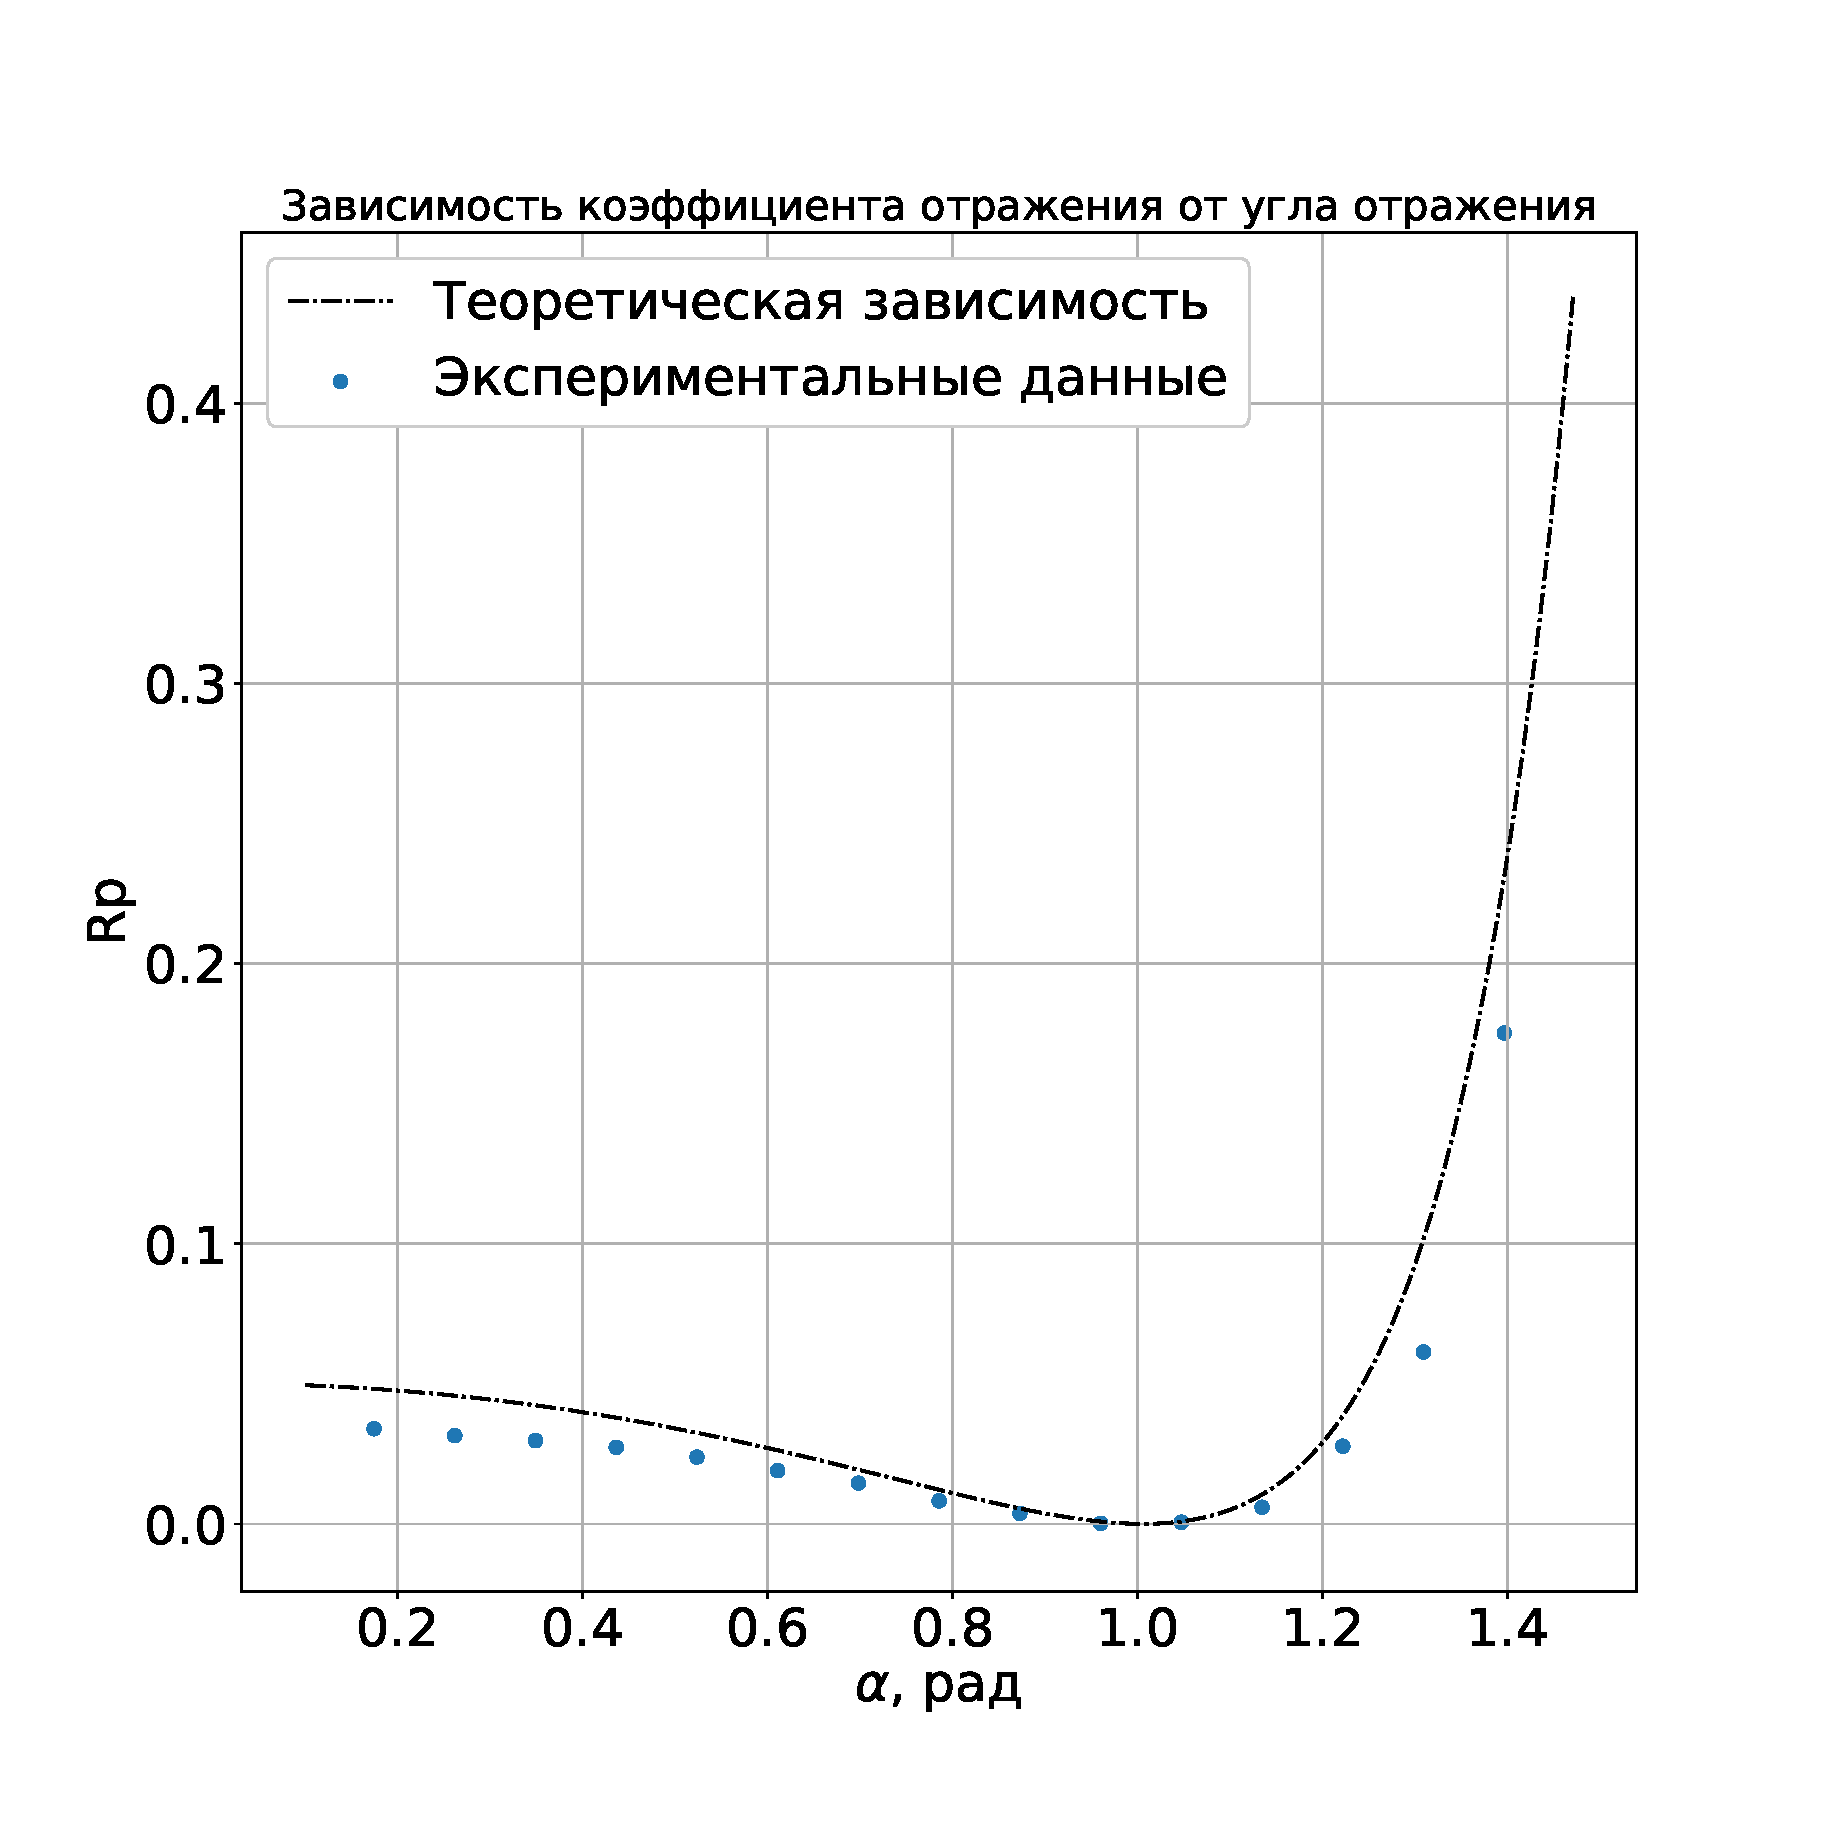
\includegraphics[width=1\linewidth]{Frenele_p.eps}
					\caption{$p$-поляризация}
					\label{fig3}
				\end{figure}
				
				\newpage
				
				\begin{figure}[h!]
					\centering
					\includegraphics[width=1\linewidth]{Frenele_s.eps}
					\caption{$s$-поляризация}
					\label{fig4}
				\end{figure}
				На графиках видно, что характер зависимости очень похож на теоретическую. Графики подгонялись по параметру $n_2$ - коэффициенту преломления в черном зеркале. Итоговые значения получились следующими:
				\begin{equation}
					\begin{cases}
						n_{p} \approx 1.58, \\
						n_{s} \approx 1.36. \\
					\end{cases}
				\end{equation}
				Что немного не входит в предел погрешностей, однако все еще лежит в $10 \%$ интервале.
				
				Кроме экспериментов с черным зеркалом, был проведен одиночный эксперимент со стеклянной пластинкой для $s$-поляризации. Результаты получились следующими:
				
				\begin{equation}
					n_s \approx 1.39
				\end{equation}
				
				Что очень хорошо сходится с результатами, полученными ранее.
	\section{Поляризация}
		\subsection{Линейный поляризатор и закон Малюса}
			\subsubsection{Постановка эксперимента}
				Для измерения поляризации источника света была использована следующая схема:
				
					\begin{figure}[h!]
						\centering
						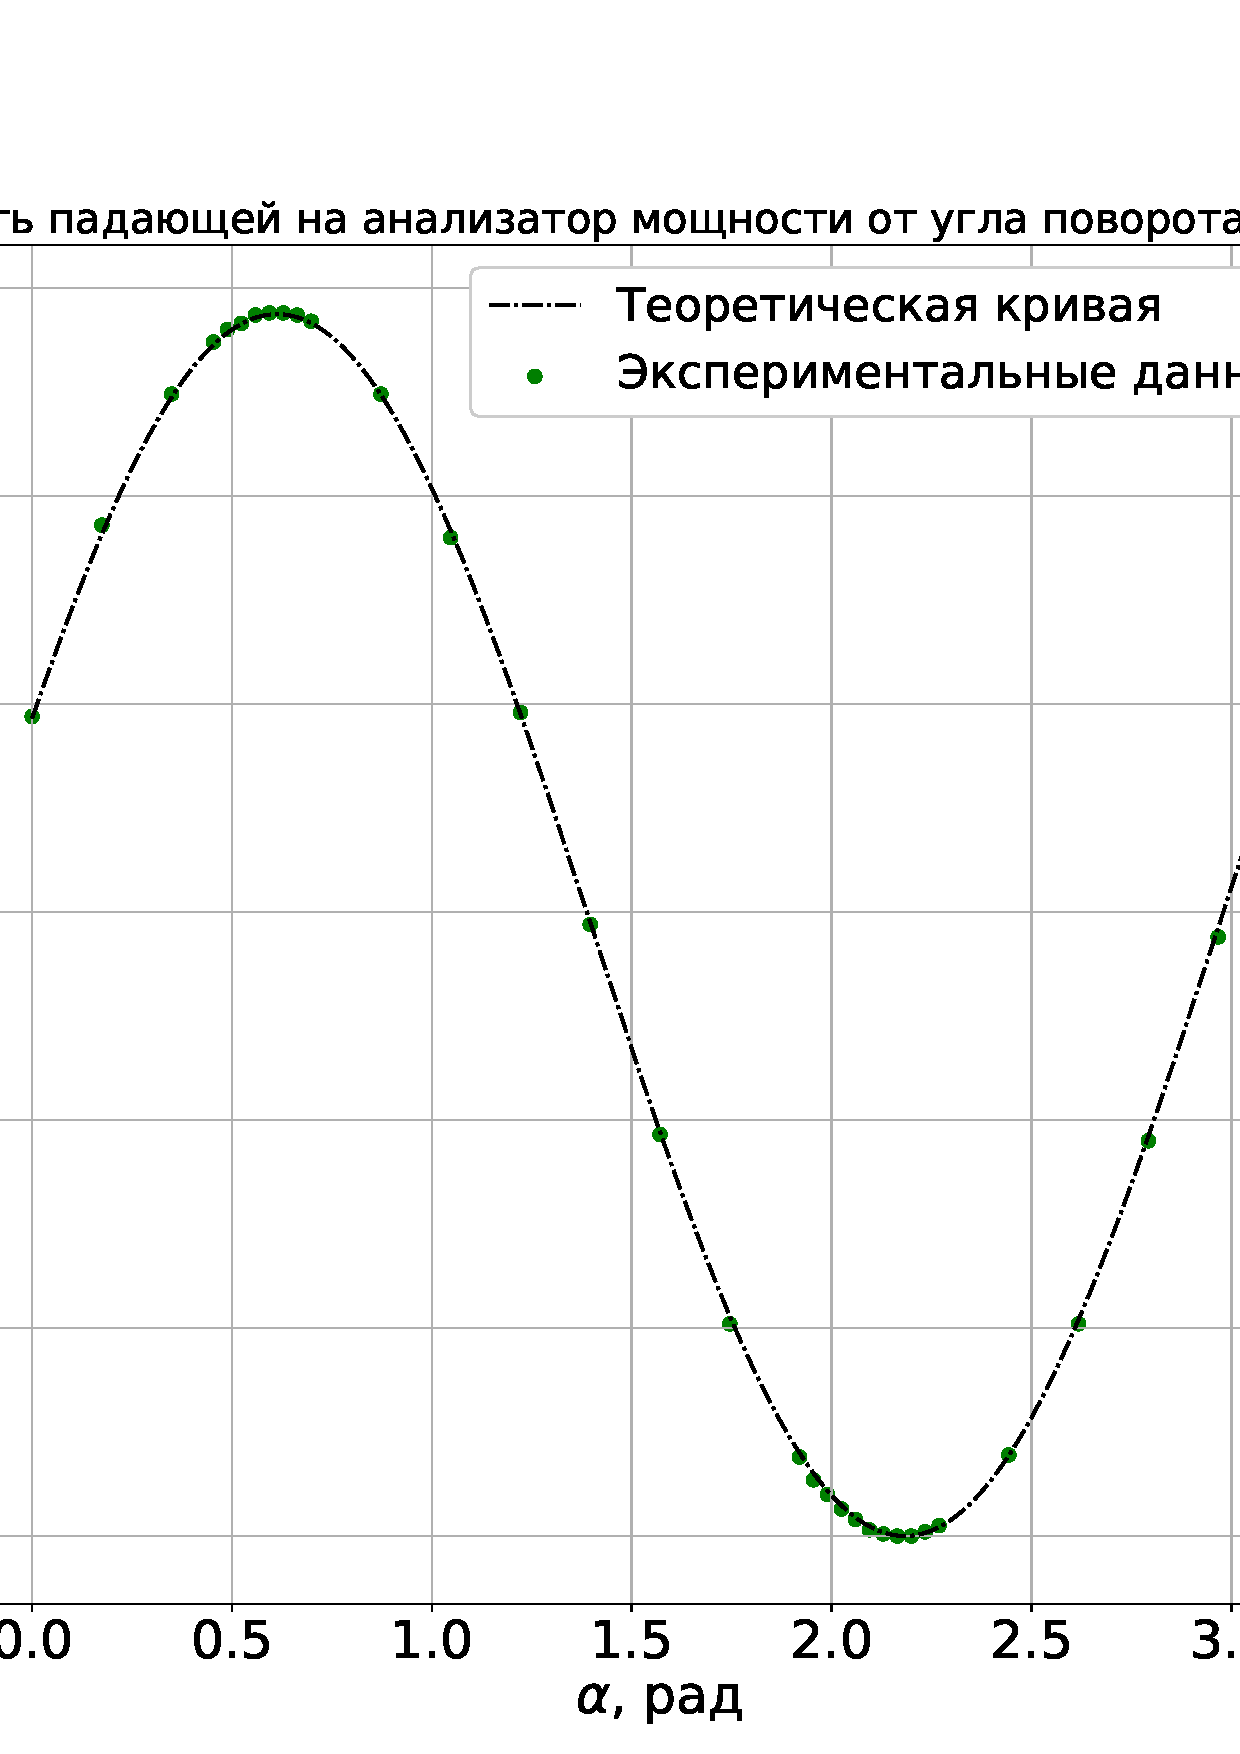
\includegraphics[width=1\linewidth]{Malus.png}
						\caption{Схематичное изображение оптической системы}
						\label{fig5}
					\end{figure}
				Здесь, вращая линейный поляризатор, можно понять, является ли источник линейно поляризованным. Если источник линейно поляризован, то при некотором угле будет наблюдаться падение интенсивности до нуля.
				
				На той же установке, доказав, что источник линейно поляризован, можно доказать справедливость закона Малюса, измерив интенсивность света при нескольких различных значениях углов
				
			\subsubsection{Результаты эксперимента}
				Получив, что интенсивность источника падает практически до нуля при некотором значении угла ориентации линейного поляризатора, мы измерили интенсивность при различных углах. Изобразим полученные результаты на графике:
				
				\begin{figure}[h!]
					\centering
					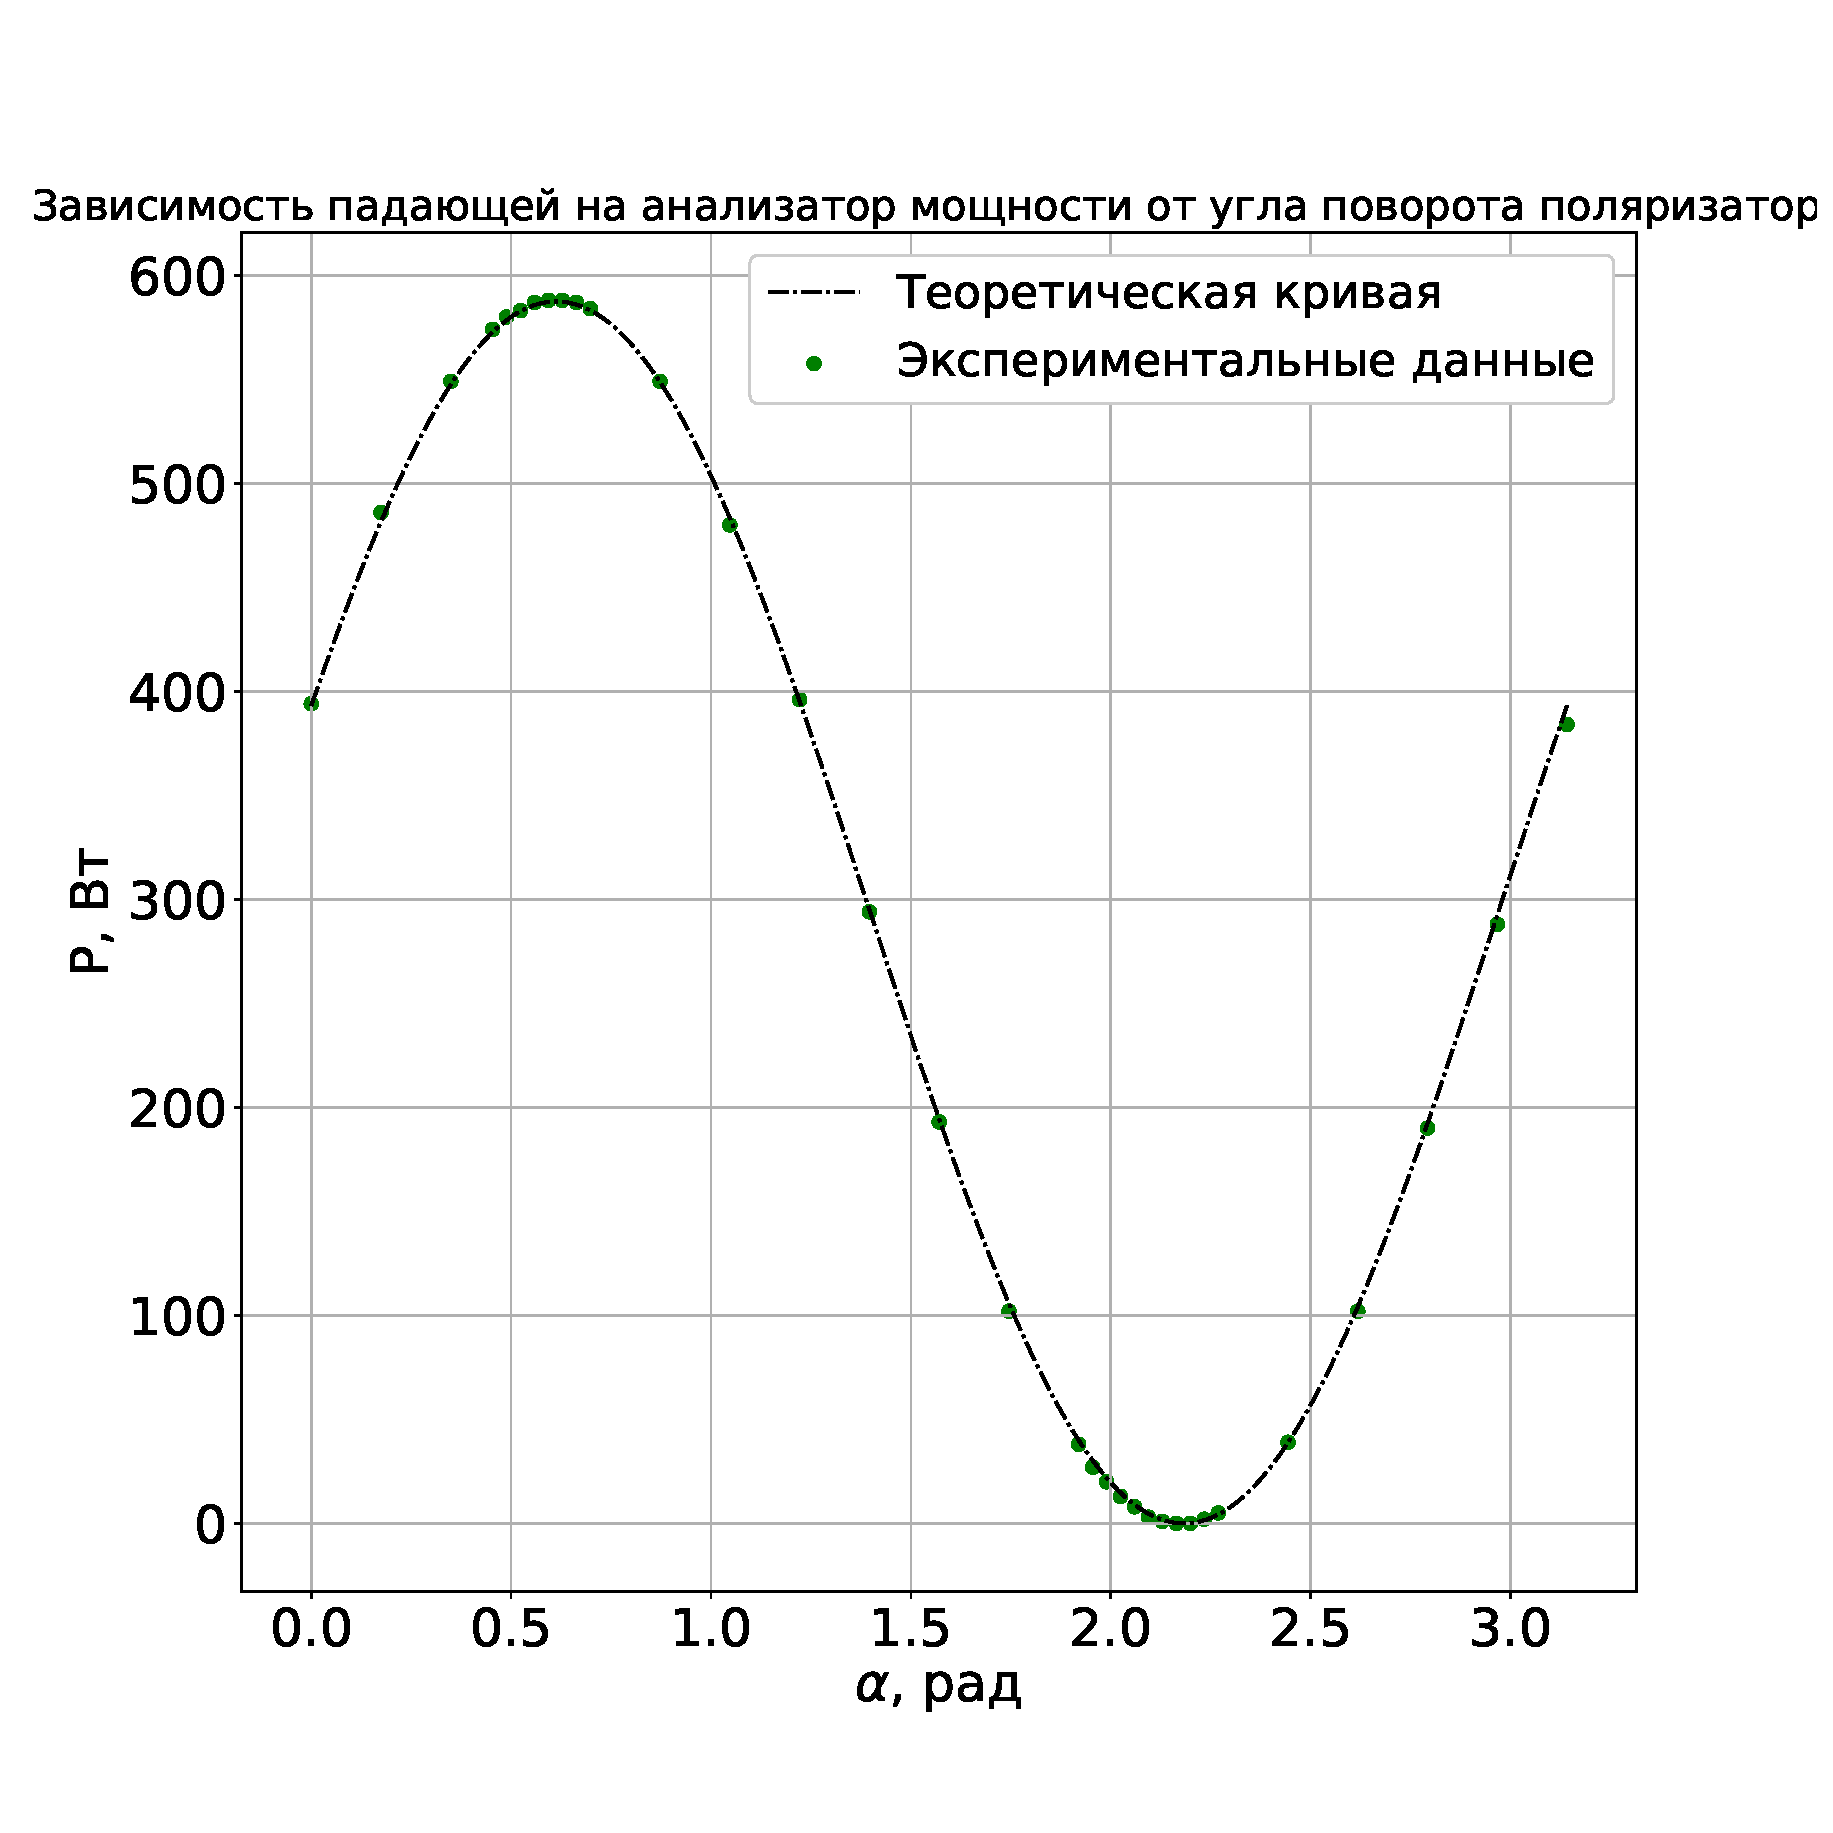
\includegraphics[width=1\linewidth]{Malus.eps}
					\label{fig6}
				\end{figure}
				
				Как можно заметить на графике, экспериментальные данные практически идеально ложатся на подогнанную теоретическую кривую, что свидетельствует о справедливости закона Малюса.
		\subsection{Пластинки $\lambda / 2$ и $\lambda /4$}
			\subsubsection{Постановка эксперимента}
				Для исследования пластинок $\lambda / 2$ и $\lambda / 4$ использовалась следующая схема:
				
				\begin{figure}[h!]
					\centering
					\includegraphics[width=1\linewidth]{Lambda.png}
					\label{fig7}
				\end{figure}
				
				Для определения главной оси полуволновой пластинки повернем линейные поляризаторы перпендикулярно друг другу (кроме этого , можем изначально повернуть первый поляризатор по главной оси, которая была найдена ранее), тогда при вращении пластинки, в некоторой точке будет наблюдаться нуль интенсивности прошедшего света (так как пластинка не поменяет направление поляризации прошедшего света), такое направление как раз будет главным.
				
				Для четвертьволновой пластинки, можно использовать ту же схему, так как в главных направлениях эллиптическая поляризация будет вырождаться в линейную. Кроме этого, можно найти такое положение поляризатора, при котором вращая второй поляризатор интенсивность света будет испытывать минимальные колебания (в идеале интенсивность будет постоянной).
				
				Для измерения степени поляризации измерялись минимумы и максимумы интенсивности при вращении второго поляризатора при постоянном угле поворота пластинки.
			\subsubsection{Результаты эксперимента}
				Степень поляризации при разных углах в четвертьволновой пластинке получилась следующей:
				\begin{equation}
					\begin{cases}
						P_{45^\circ} \approx 0.07, \\
						P_{30^\circ} \approx 0.34, \\
						P_{60^\circ} \approx 0.49. \\
					\end{cases}
				\end{equation}
				
				Отсюда видно, что поляризатор не идеален, так как в идеальном поляризаторе $P_{45^\circ} = 0$. Тем не менее, наблюдается эллиптическая поляризация, что соответствует четвертьволновой пластинке.
				
				Чтобы определить какая именно перед нами пластинка, необходимо использовать ту же схему, и при нескольких углах поворота пластинки вращать второй поляризатор. Полуволновая пластинка при некотором угле поворота поляризатора будет давать нулевую интенсивность на выходе. Четвертьволновая пластинка будет иметь минимум и максимум, но не нуль (для точности результата, предлагается сделать измерения при нескольких углах поворота четвертьволновой пластинки, отличающихся на не кратный $\pi / 2$ угол, чтобы точно не попасть в главную ось)
				
	\section{Выводы}
		\begin{itemize}
			\item Нами были изучены поляризаторы разных видов (линейные и эллиптические)
			\item Нами были получены значения угла Брюстера для стеклянной пластинки и черного зеркала, а также коэффициенты , эти значения оказались близки к теоретическим, что позволяет судить о справедливости формул Френеля
			\item Была проверена справедливость закона Малюса, теоретическая кривая очень хорошо описывает экспериментальные данные.
			\item Мы исследовали поведение поляризованного света при прохождении через пластинки $\lambda / 2$ и $\lambda / 4$. Определили степени поляризации при различных углах ориентации пластинок
		\end{itemize}
\end{document}